\chapter{Structure of Multiple-Electron Atoms}



\section{Identical Particles}

\subsection{Direct Sums and Direct Products of States}\label{direct sum}

For two quantum states in their Hilbert spaces, 
there are multiple ways to combine them and desribe the overall system as one total wave function according to their relation:

\subsubsection{Superposition}

If the states, generally orthonormal, reside in the same space, the total wavefunction is a \emph{superposition state} written as their linear combination. The overall state collapse into one of the components upon observation according to their probability distribution:
\[
\ket{\psi} = \sum_{n}c_n\ket{\psi_n},
\quad\sum_{n}|c_n|^2=1\text{ for normalization}
\]

\subsubsection{Direct Sum}

For two distinct, or mathematically orthogonal spaces, along with the states in them, their \emph{direct sum} is an extended space spanned by the union of their basis vectors. A state reside in one component only, mutually exclusive, reflecting \emph{classical alternatives} but not quantum superposition:
\[V_{AB} = V_A \oplus V_B, \quad \dim V_{AB} = \dim V_A + \dim V_B\]

\subsubsection{Direct Product}

For two distinct spaces, their \emph{direct product} forms a composite space by combining the degrees of freedom of the subspaces. 
It is like putting two parts of a system together to get a complete one, e.g.
$\ket{\text{spin}} \otimes \ket{\text{position}} = \ket{\text{particle state}}$
\[V_{AB} = V_A \otimes V_B, \quad \dim V_{AB} = \dim V_A \cdot \dim V_B\]


\subsection{Quantum Entanglement}\label{entangle}

For two non-interacting particles (even those that can pass through each other), with potential $V(\mathbf{r}_1, \mathbf{r}_2) = V(\mathbf{r}_1) + V(\mathbf{r}_2)$, the total wavefunction is a linear combination of direct products of individual states:
\[
\Psi = \sum_{k}c_{k}\ket{a_k}_1\otimes\ket{b_k}_2
=\sum_{k} c_{k} \psi_{ak}(\mathbf{r}_1)\psi_{bk}(\mathbf{r}_2)
\]
These two expression are identical, meaning that particle 1 is in state $a_k$ and particle 2 in $b_k$.\\ \\
At this point, the states of $\mathbf{r}_1$ and $\mathbf{r}_2$ are correlated: if observation determines that particle 1 is in state $a_m$, then regardless of the coefficient $c_m$, particle 2 must be in state $b_m$.
The correlation arising from \textit{first taking the direct product then superposing} is called \emph{quantum entanglement}.

\subsubsection{Separable vs. Entangled States}

In the direct product space $\mathcal{H}_A \otimes \mathcal{H}_B$, consider a general state:
\[
    \ket{\Psi}_{AB} = \sum_{ij} c_{ij} \ket{i}_A \otimes \ket{j}_B
\]
A state is \emph{separable} if the state can be \emph{factorized}:
\[
    \ket{\Psi}_{AB} = \ket{\psi}_A \otimes \ket{\phi}_B
\]
where $\ket{\psi}_A$ and $\ket{\phi}_B$ are superpositions of each particle's own state:
\[
\ket{\psi}_A = \sum_{i}a_i\ket{\psi_i}_A, \quad 
\ket{\phi}_B = \sum_{j}b_j\ket{\psi_j}_B
\]
i.e., the coefficient matrix $c_{ij}$ has rank 1: $c_{ij} = a_i b_j$, because thus measuring particle $A$ will give result in accordance to $\ket{\psi}_A$ with nothing to do with particle $B$, and vice versa, suggesting that they are not correlated.\\
Hence if a state cannot be factorized, the two particles are \emph{entangled}, which, as described, occurs that measurement of particle $A$ instantaneously determines the state of particle $B$, regardless of distance.

\subsubsection{Schmidt Decomposition}

We shall formalize the discussion we did: any bipartite pure state can be written in its \emph{Schmidt form}:
\[
\ket{\psi} = \sum_{k=1}^{r}\lambda_k\ket{u_k}_A\otimes\ket{v_k}_B,
\quad \sum_{k}\lambda_k^2=1
\]
We name $r$ \emph{degree of entanglement}, so that $r=1$ for a separable state, and $r>1$ an entangled state.\\
Calling back on \ref{entangle2}, for the singlet state of two electrons: $\lambda_1 = \lambda_2 = 1/\sqrt{2}$, so $r = 2$ which is the maximal entanglement for two-level systems.

\subsection{Bosons and Fermions}
If two identical particles occupy states $a$ and $b$ respectively, and since they are indistinguishable, the probability of finding them in states $a$ and $b$ is equal. The wavefunction is a linear combination of both configurations:
\[
    \Psi_{\pm}(\mathbf{r}_1, \mathbf{r}_2) = \frac{1}{\sqrt{2}}\left[\psi_a(\mathbf{r}_1)\psi_b(\mathbf{r}_2) \pm \psi_a(\mathbf{r}_2)\psi_b(\mathbf{r}_1)\right]
\]
Both combinations ensure normalization and equal probability (the factor $1/\sqrt{2}$ accounts for the orthonormality of different wavefunctions under the same label), but plus and minus are different:

\begin{itemize}
    \item When taking the + sign: The wavefunction is symmetric under particle exchange. We name these particles \emph{bosons}.
    \item When taking the - sign: The wavefunction is antisymmetric under particle exchange. We name these particles \emph{fermions}.
\end{itemize}
Bosons have integer spins while fermions have half-integer spins.

\subsubsection{Pauli exclusion principle}\label{pauli}

According to definition, two fermions cannot occupy the same state; otherwise the total wavefunction vanishes:
\[
    \Psi = \frac{1}{\sqrt{2}}\left[\psi_a(\mathbf{r}_1)\psi_a(\mathbf{r}_2) - \psi_a(\mathbf{r}_2)\psi_a(\mathbf{r}_1)\right] = 0
\]
Which is the \emph{Pauli exclusion principle} of fermions.

\subsection{Exchange Energy}

For distinguishable particles with particle 1 in state $\ket{a}$ and 2 in $\ket{b}$, the expectation of separation is given by:
\[
    \langle (x_1 - x_2)^2 \rangle = \langle x_1^2 \rangle + \langle x_2^2 \rangle - 2\langle x_1 x_2 \rangle = \langle x^2 \rangle_a + \langle x^2 \rangle_b - 2\langle x \rangle_a \langle x \rangle_b
\]
(for the computation of expectations, see \ref{expectation}.)\\
However, for identical particles:
\[
\langle x_1^2 \rangle = \langle x_2^2 \rangle = \frac{1}{2}(\langle x^2 \rangle_a + \langle x^2 \rangle_b)
\]
The matrix element is denoted as $\expect{x}_{ab} = \bra{a}x\ket{b}$, so that:
\[
    \langle (x_1 - x_2)^2 \rangle = \langle x^2 \rangle_a + \langle x^2 \rangle_b - 2\langle x \rangle_a \langle x \rangle_b \mp 2|\langle x \rangle_{ab}|^2
\]
Due to particle indistinguishability, an extra term $2|\expect{x}_{ab}|^2 > 0$ appears. Thus:
\begin{itemize}
    \item For fermions with a minus sign: Equivalent particles are farther apart than distinguishable particles;
    \item For bosons with a plus sign: Equivalent particles are closer together.
\end{itemize}
For electrons (fermions), the antisymmetric spatial wavefunction keeps them farther apart, reducing electrostatic repulsion energy. This energy reduction is called \emph{exchange energy}.


\section{Spin and Total Wavefunction}
\subsection{Hund's First Rule}

The state of a particle consists of spatial and spin parts:
\[
    \Psi(\mathbf{r}_1, \mathbf{r}_2, \ldots, \mathbf{r}_n) = \psi(\mathbf{r}_1, \mathbf{r}_2, \ldots, \mathbf{r}_n) \otimes \chi(\mathbf{r}_1, \mathbf{r}_2, \ldots, \mathbf{r}_n)
\]
The antisymmetry requirement under exchange of any two particles:
\[
    \Psi(\ldots, \mathbf{r}_i, \ldots, \mathbf{r}_j, \ldots) = -\Psi(\ldots, \mathbf{r}_j, \ldots, \mathbf{r}_i, \ldots)
\]
To ensure overall antisymmetry, either the spatial part or the spin part must be antisymmetric (but not both). Since spatial antisymmetry reduces Coulomb energy via exchange interaction, spins tend to align parallel, which leads to \emph{Hund's first rule}: Under the Pauli principle, the state with maximum spin has the lowest energy.

\subsection{Slater Determinant}\label{slater det}

Consider a system with two electrons in two states: one spacial state $\psi$ and two spin states $\alpha$ and $\beta$.
Hence there's one ovreall spacial state, and recalling \ref{entangle2}, there're four spin states at all:
\[\begin{aligned}
&\text{Spacial part: }&\psi(1)\psi(2)\\
&\text{Spin part: }&\alpha(1)\alpha(2), \quad\beta(1)\beta(2), \quad\frac{1}{\sqrt{2}}[\alpha(1)\beta(2)\pm\alpha(2)\beta(1)]
\end{aligned}\]
In order to satisfy antisymmetry requirement, of the four possible combinations only the singlet state is valid as the spacial part is symmetrical.
The total state can then be written in form of a determinant.
\[
\Psi = \frac{1}{\sqrt{2}}\psi(1)\psi(2)[\alpha(1)\beta(2)-\alpha(2)\beta(1)] = 
\frac{1}{\sqrt{2}}
\begin{vmatrix}
\psi(1)\alpha(1) & \psi(2)\alpha(2) \\
\psi(1)\beta(1)  & \psi(2)\beta(2)
\end{vmatrix}
\]
Similarly, for a system of $N$ identical fermions, 
the antisymmetric wavefunction with in all $N$ spacial $\otimes$ spin states can be elegantly written as a \emph{Slater determinant}:
\[
    \Psi(1,2,\cdots,N) = \frac{1}{\sqrt{N!}}
    \begin{vmatrix}
        \psi_a(1)\alpha(1) & \psi_a(2)\alpha(2) & \cdots & \psi_a(N)\alpha(N) \\
        \psi_a(1)\beta(1)  & \psi_a(2)\beta(2)  & \cdots & \psi_a(N)\beta(N)  \\
        \vdots & \vdots & \ddots & \vdots \\
        \psi_z(1)\beta(1)  & \psi_z(2)\beta(2)  & \cdots & \psi_z(N)\beta(N)
    \end{vmatrix}
\]

\section{Electronic Structure of Many-Electron Atoms}
(Applicable to ground-state atoms in gas phase)

\subsection{Penetration and Shielding}

Electron-electron repulsion can be viewed as shielding of nuclear charge. Electrons have probability to enter smaller-radius orbits, experiencing less shielding and greater nuclear attraction (penetration), lowering energy. Once inside, they shield other electrons.\\
As discussed in \ref{node}, when principal quantum number $n$ are equal, the smaller $l$, the more radial nodes and distribution probability peaks nearer to the nucleus:
\begin{figure}[h]
\centering
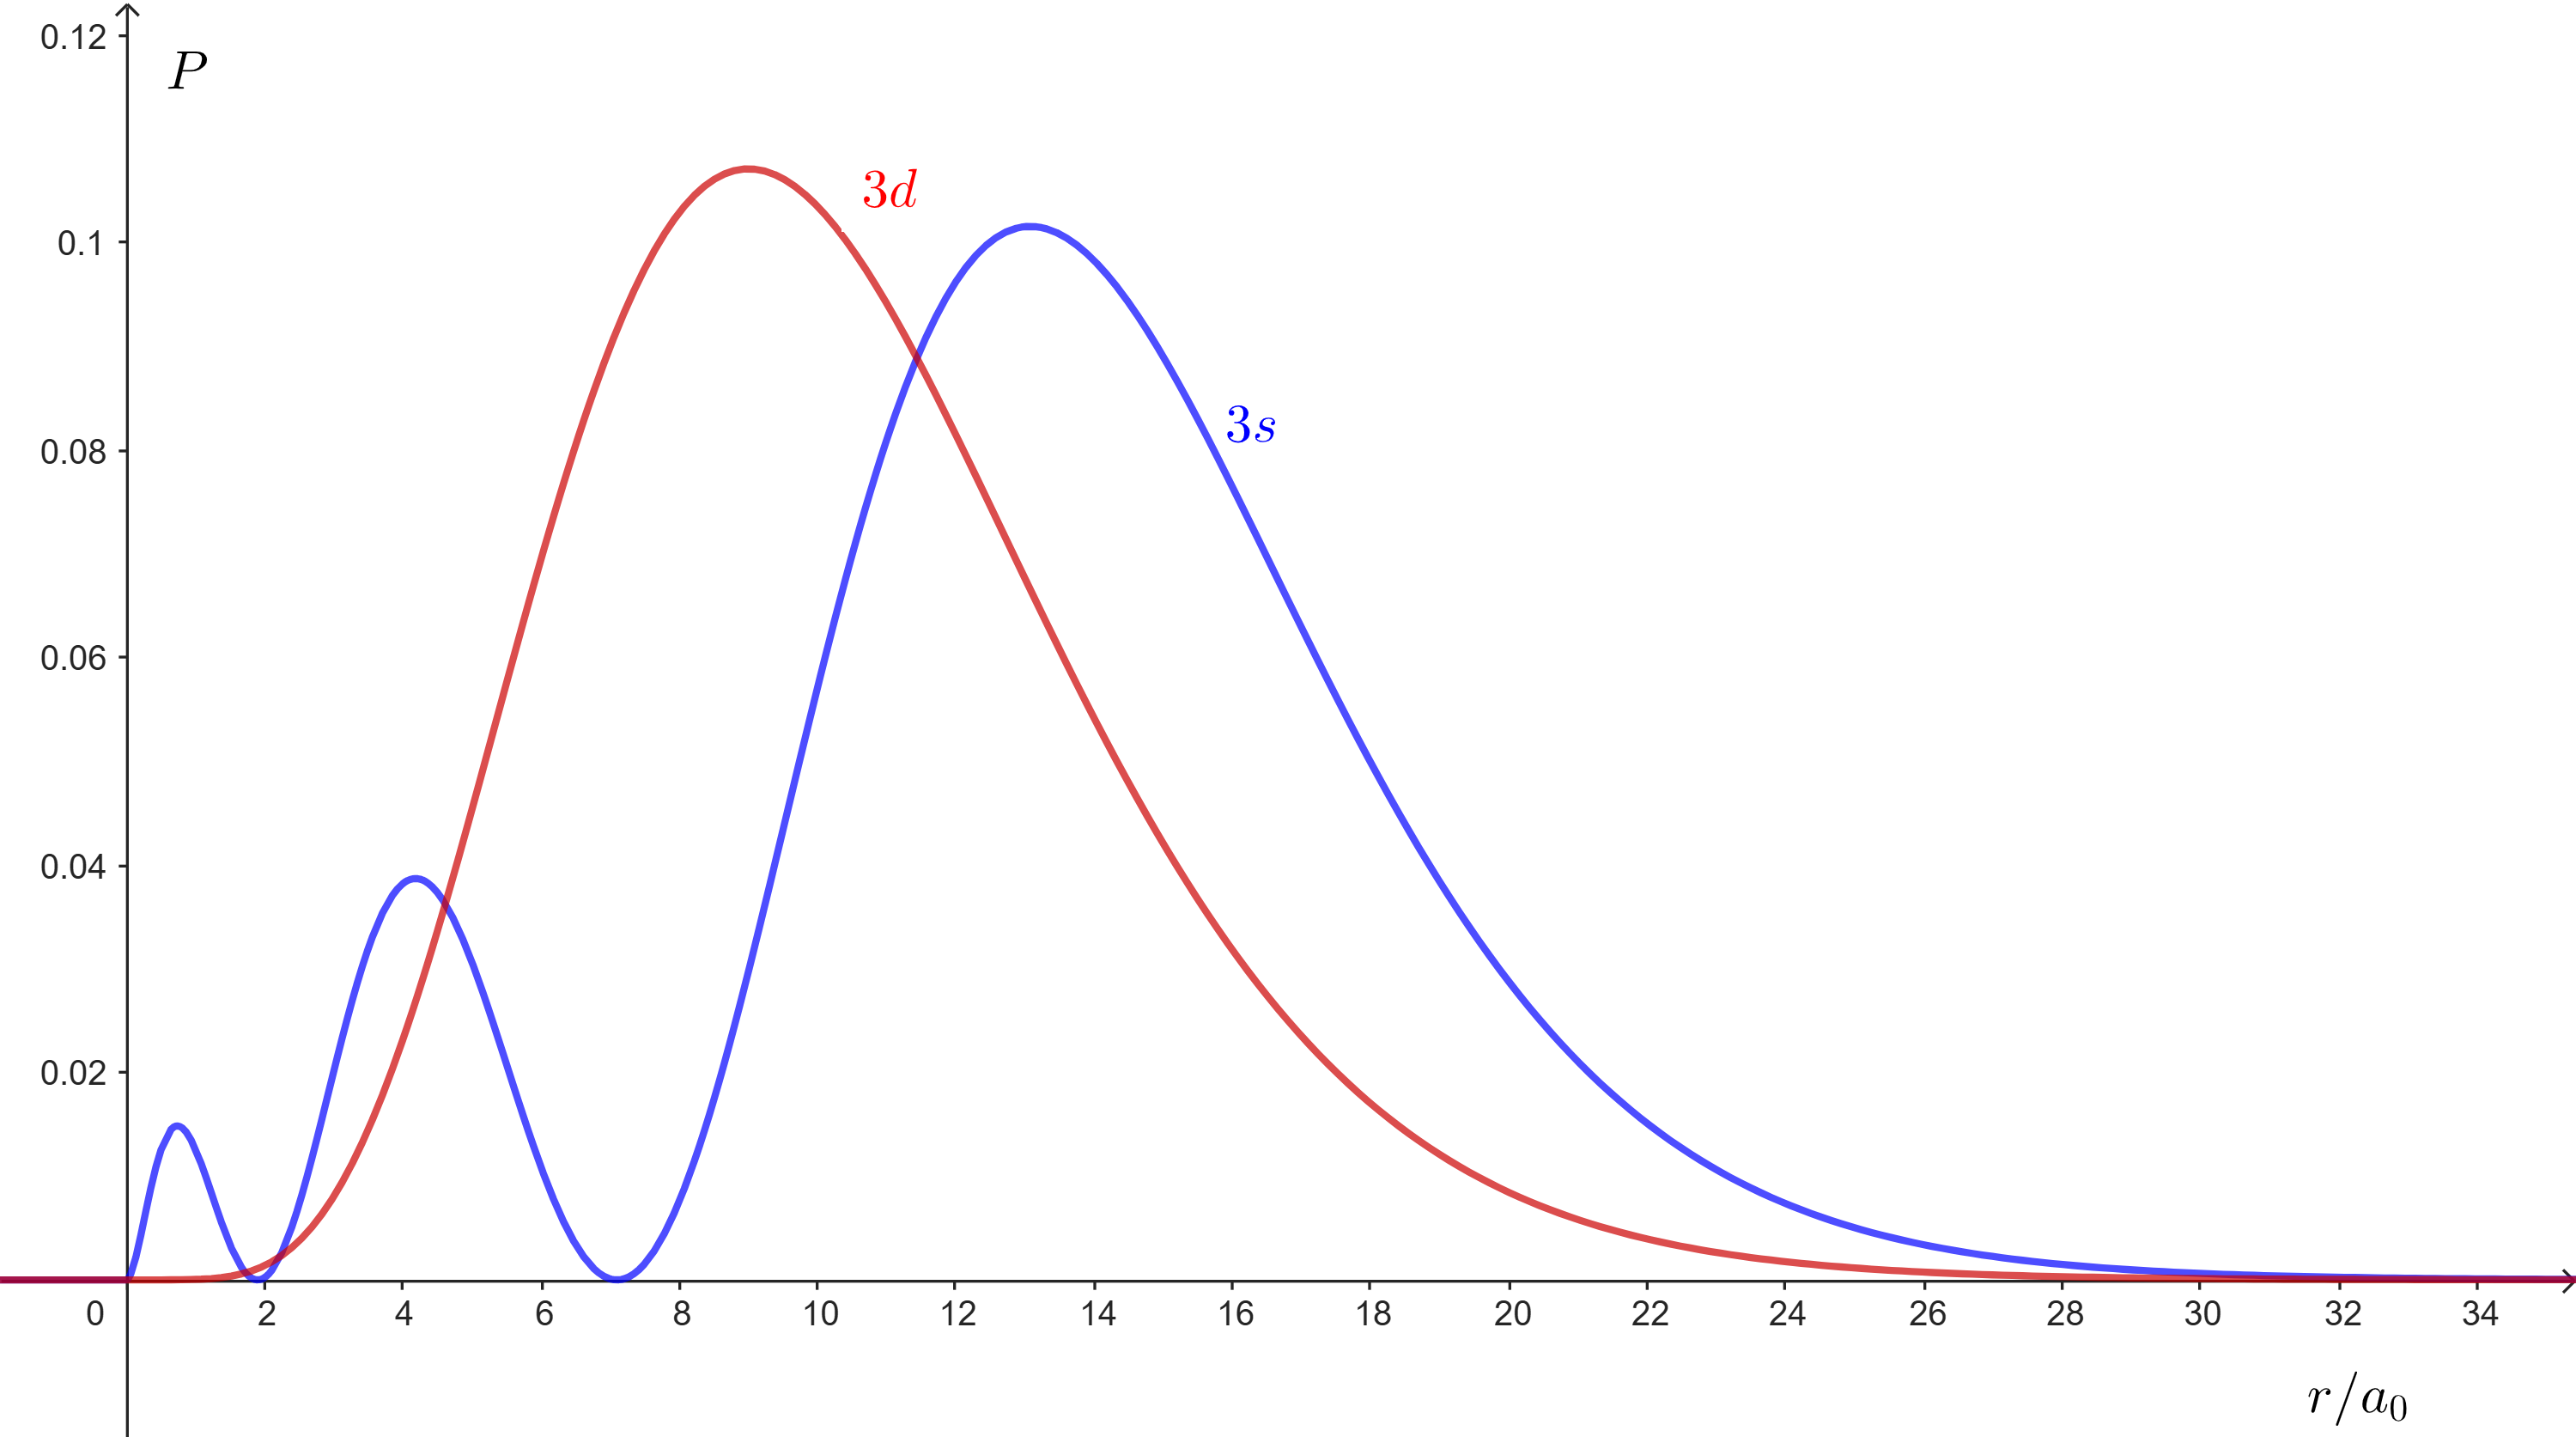
\includegraphics[scale=0.3]{Ch5/penetration}
\caption{Radial distribution functions of 3s and 3d orbital}
\end{figure}
Therefore, when principal quantum numbers are equal:
\begin{itemize}
    \item s orbitals: Probability peak near nucleus leads to strong penetration and shielding;
    \item d, f orbitals: Small probability near nucleus, shielded by s, p orbitals: weak penetration and shielding.
\end{itemize}
So penetration/shielding ability: $s > p > d > f$, therefore energy: $s < p < d < f$.

\subsection{Subshell Filling}

Electrons generally follows the \emph{building-up principle}: fill subshells in order of increasing energy when occupying molecular orbitals.\\ \\
However, for $d$ and $f$ orbitals their electron capacity is large, 
but they have fewer peaks in radial distribution relative to $s$ and $p$ orbitals, 
leading to a more crowded occupation of electrons. 
Therefore, for atoms with partially filled $d$ or $f$ subshells, electrons often occupy higher orbitals first to relieve intra-subshell repulsion, 
giving rise to what called state crossing. When forming compounds, 
these higher-energy electrons are lost first due to decreased radius and thus larger electrostatic attraction.
\[\text{Typically, d-block }(n+1)s^2 nd^x\text{ and f-block }(n+2)s^2 (n+1)d^1 nf^x\]
\begin{figure}
\centering
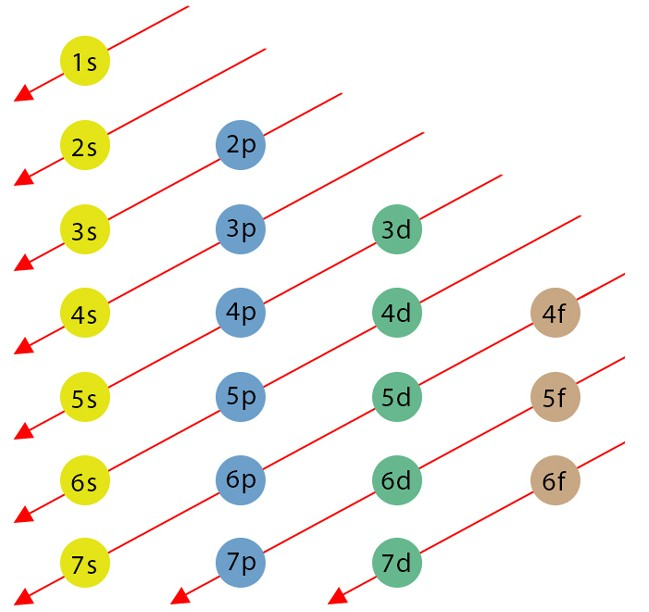
\includegraphics[scale=0.35]{Ch5/afbau}
\caption{Energy order of subshells}
\end{figure}
Additionally, due to the extra stability of half-filled (maximum exchange energy) or fully-filled (best spherical symmetry) configurations, 
some elements disobey the building-up principle to achieve them (e.g., Cr: $[Ar]3d^54s^1$, Cu: $[Ar]3d^{10}4s^1$).

\subsection{Spin-Orbit Coupling and Term Symbols}\label{spectral term}

Due to spin-orbit coupling (proportional to $Z^4$, see \ref{soc}), each subshell splits into different energy levels (microstates) when filling electrons.
Within a same subshell, complement electronic configurations have the same spectral terms with the opposite order.

\subsubsection{LS Coupling}
For light atoms with small $Z$, spin-orbit coupling is not significant for a single electron within its orbital. Therefore the angular momenta of electrons and orbitals each adds up first, and then the total spin and total orbital interacts:
\begin{align*}
    \mathbf{L} &= \sum \mathbf{l}_i  {}&(L = |l_1 + l_2|, \ldots, |l_1 - l_2|) \\
    \mathbf{S} &= \sum \mathbf{s}_i  {}&(S = |s_1 + s_2|, \ldots, |s_1 - s_2|) \\
    \mathbf{J} &= \mathbf{L} + \mathbf{S}  {}&(J = |L+S|, \ldots, |L-S|)
\end{align*}
The states with different $L$, $S$ and $J$ can be expressed in \emph{term symbols}: $\boxed{{}^{2S+1}L_J}$ where $L$ is denoted S, P, D, F, G,...

\subsubsection{jj Coupling}

For heavy atoms with large $Z$, each electron first couples its own orbital and spin angular momenta:
\[
    \mathbf{j}_i = \mathbf{l}_i + \mathbf{s}_i
\]
Then total $\mathbf{J} = \sum \mathbf{j}_i$.

\subsubsection{Selection Rules}

Electric dipole transitions (LS coupling):
\[
    \Delta S = 0, \quad \Delta L = 0, \pm 1, \quad \Delta l = \pm 1, \quad \Delta J = 0, \pm 1 \text{ (but } J=0 \nleftrightarrow J=0\text{)}
\]

\subsection{Ground State Microstates and Hund's Rules}

\begin{enumerate}
    \item Hund's first rule: Maximum $S$ maximizes exchange energy reduction, so spins parallel first than pairing.
    \[
        S = \sum m_{s,\text{max}}
    \]
    
    \item Hund's second rule: For given $S$, maximize $L$ to minimize Coulomb repulsion as electrons orbit in same direction, avoiding each other.
    \[
        L = \sum m_{l,\text{max}}
    \]
    
    \item Hund's third rule: Minimum $J$ for less than half-filled, maximum $J$ for more than half-filled to increase spin-orbit coupling
    \[
        J = |L \pm S|,\text{ (Minus for less than half-filled, plus for more than half-filled)}
    \] 
\end{enumerate}
Example: Vanadium $[Ar]4s^23d^3$
\begin{align*}
    m_s &: \uparrow\ \uparrow\ \uparrow \quad \Rightarrow \quad S_{\text{max}} = \frac{3}{2} \\
    m_l &: +2, +1, 0 \quad \Rightarrow \quad L_{\text{max}} = 3
\end{align*}
Less than half-filled $\Rightarrow J_{\text{min}} = L - S = \frac{3}{2}$.\\
Term symbol: $\boxed{{}^4\!F_{3/2}}$\\
As a quick side note, Hund's rule can only predict ground state spectral term, but cannot rank the order of excited states. \\


\section{Atomic Radius}

Atomic radius refers to metallic radius or covalent radius for nonmetals.
\begin{itemize}
    \item Across a period: Increasing nuclear charge with incomplete shielding $\Rightarrow$ increasing effective nuclear charge $\Rightarrow$ radius decreases
    \item Down a group: Increasing principal quantum number dominates $\Rightarrow$ radius increases
\end{itemize}
The trend of electronegativity and most periodicities can be explained similarly, 
ascribing to the change of effective nuclear charge to the outermost layer.

\subsection{Lanthanide Contraction}\label{radius}

Poor shielding by f-electrons causes 6s electrons to experience higher $Z_{\text{eff}}$, 
and the insertion of 14 f-block elements contributes to another 14 steps of radius decrease, 
causing sixth period elements being smaller than expected, giving rise to similar radii and properties of fifth and sixth period transition metals.\\
Of course the insertion of d-block elements gives similar but weaker results but we rarely mention it.   

\subsection{Relativistic Contraction}

For heavy elements ($Z \geq 70$), relativistic effects become significant:
s and p electrons (especially 1s) move at relativistic speeds, so
mass increase leads to orbital contraction (greater relativistic correction energy),
which enhanced shielding so that d and f orbitals expand,
and as a result, outer s and p electrons penetrate more, experience higher $Z_{\text{eff}}$.\\
Overall effect: Atomic radius reduced by $\sim 20\%$ for heavy elements.

\subsection{Inert Pair Effect}

Due to lanthanide and relativistic contraction, outer 6s electrons are tightly bound in heavy p-block elements (Tl, Pb, Bi). This makes the $ns^2$ pair less available for bonding, leading to oxidation states 2 less than group maximum (e.g., Tl$^+$ instead of Tl$^{3+}$).